% VUT FIT MITAI
% MSZ 2021/2022
% Author: Vladimir Dusek
% Login: xdusek27

%%%%%%%%%%%%%%%%%%%%%%%%%%%%%%%%%%%%%%%%%%%%%%%%%%%%%%%%%%%%%%%%%%%%%%%%%%%%%%%%

% Path to figures
\graphicspath{{avs/architektury_se_sdilenou_pameti/figures}}

%%%%%%%%%%%%%%%%%%%%%%%%%%%%%%%%%%%%%%%%%%%%%%%%%%%%%%%%%%%%%%%%%%%%%%%%%%%%%%%%

\chapter{AVS~--~Architektury se sdílenou pamětí UMA a NUMA, zajištění lokality dat.}

%%%%%%%%%%%%%%%%%%%%%%%%%%%%%%%%%%%%%%%%%%%%%%%%%%%%%%%%%%%%%%%%%%%%%%%%%%%%%%%%

\section{Zdroje}

\begin{compactitem}
    \item \path{AVS-11.pdf}
    \item \path{AVS-12.pdf}
    \item \path{AVS_2019-12-02.mp4}
    \item \path{AVS_2019-12-09.mp4}
\end{compactitem}

%%%%%%%%%%%%%%%%%%%%%%%%%%%%%%%%%%%%%%%%%%%%%%%%%%%%%%%%%%%%%%%%%%%%%%%%%%%%%%%%

\section{Architektury se sdíleným adresovým prostorem}

\begin{compactitem}
    \item Jaký potřebujeme hardware aby nám fungovala správně sdílená paměť, která je potřebná pro paralelizaci.

    \item Sdílený adresový prostor (SAS, \textit{shared address space}).

    \item Sekvenční počítač: \begin{compactitem}
        \item Vidí vlastní čtení a zápisy v pořadí, jak je vydává.
        \item Při čtení vidí poslední hodnotu zapsanou na danou adresu.
        \item U paralelního počítače ale různé CPU nemusí vidět paměťové akce ve stejném pořadí.
    \end{compactitem}

    \item U paralelního počítače musíme zajistit: \begin{compactitem}
        \item \textbf{Šíření zápisů} -- každý zápis se stane viditelný všem CPU, tj. všem jádrům.
        \item \textbf{Serializaci zápisů} -- všechny CPU vidí zápisy na adresu x v témže pořadí (u sběrnice splněno triviálně).
    \end{compactitem}

    \item Jakmile do sdílené paměti může přistupovat více vláken, je nutné zajistit, aby na jedné adrese našla při čtení vždy stejná data, ať jsou data v kterékoliv úrovni cache nebo v hlavní paměti (tj. koherentní kopie).

    \item \textbf{Koherence} se týká jednoznačnosti zápisů/čtení na 1 adresu.

    \item \textbf{Konzistence} se týká pořadí přístupů na různé adresy. Oproti koherenci specifikuje v jakém pořadí jednotlivé procesy spouštějí své paměťové operace, či jak se toto pořadí jeví ostatním procesům.
\end{compactitem}

\subsection{UMA (\textit{uniform memory access})}

\begin{compactitem}
    \item Uniformní doba přístupu do hlavní paměti. \begin{compactitem}
        \item Každý procesor/jádro platí stejnou pokutu za přístup do libovolné části paměti.
    \end{compactitem}

    \item Implementace: \begin{compactitem}
        \item Plné propojení -- extrémně drahé.
        \item Sběrnice -- jedna sběrnice o kterou procesory soupeří, neefektivní.
        \item Křížový přepínač (X-bar) -- umožňuje paralelní přenosy.
        \item Kruhové propojení -- lepší než sběrnice, levnější než křížový přepínač.
        \item Propojovací síť.
    \end{compactitem}

    \begin{figure}[H]
        \centering
        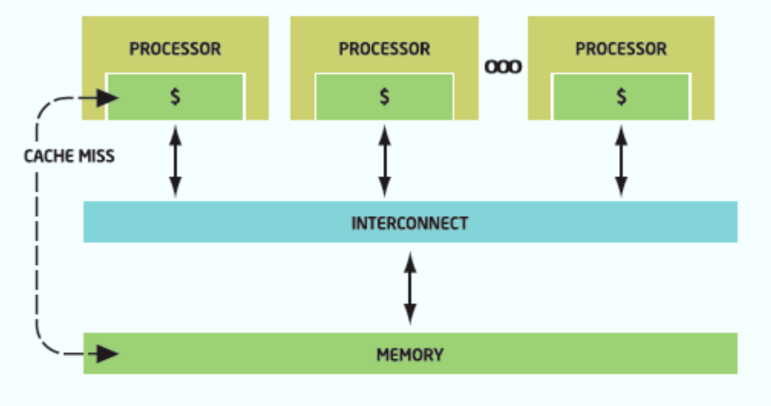
\includegraphics[width=0.9\linewidth]{uma.png}
        \caption{Architektura UMA.}
    \end{figure}
\end{compactitem}

\subsection{NUMA (\textit{non-uniform memory access})}

\begin{compactitem}
    \item Neuniformní doba přístupu do hlavní paměti (např. lokální a vzdálený výpadek v cache).

    \item Vzdálený přístup -- automatické zaslání zprávy tam a zpět.

    \item Sdílená paměť fyzicky distribuovaná $\rightarrow$ NUMA.

    \item Implementace: \begin{compactitem}
        \item Propojovací síť, např. 2D-torus, tlustý strom, hyperkostka.
        \item Někdy oddělená adresová a datová síť.
        \item Rozšiřitelnost až do 2048 jader a 64 terabajtů (TB).
    \end{compactitem}

    \begin{figure}[H]
        \centering
        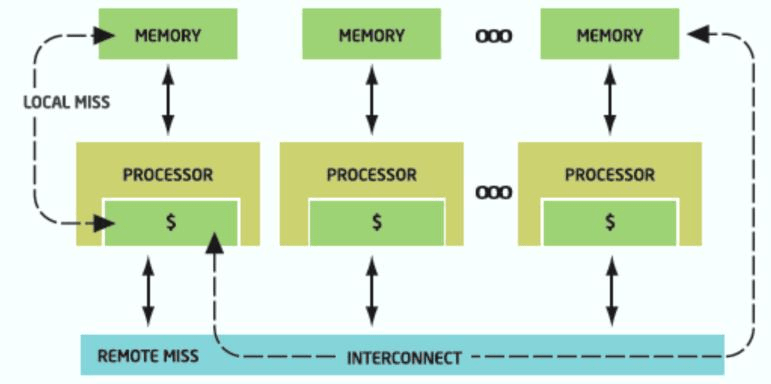
\includegraphics[width=0.9\linewidth]{numa.png}
        \caption{Architektura NUMA.}
    \end{figure}
\end{compactitem}

%%%%%%%%%%%%%%%%%%%%%%%%%%%%%%%%%%%%%%%%%%%%%%%%%%%%%%%%%%%%%%%%%%%%%%%%%%%%%%%%

\section{Zajištění lokality dat}

\begin{compactitem}
    \item \todo{Todo: dokoncit tuto sekci}
    \item \todo{Todo: koherence pameti cache na toto navazuje, viz dalsi otazka}

    \item Hlavní příčinou pomalého běhu aplikací v systému SAS je fyzická vzdálenost paměti od procesoru, který s ní pracuje.

    \item Pro uspokojivý provoz aplikace je třeba klást zvláštní důraz na zajištění lokality dat zpracovávaných dat.

    \item Případně omezení současného přepisování konkrétní stránky paměti v cache.

    \item Příklad: místo toho, aby procesor přistupoval k rychlé systémové sběrnici, aby mohl do paměti RAM, musí jít do karty PCI a pak přes dráty do přepínače, odtud do sousedního uzlu, do paměti a zpět.
\end{compactitem}
